\documentclass[12pt,a3paper]{article}
\usepackage{better_poster}
% ---- fill in from here
% authors
\title{MATS: The Next Generation Building Blocks}
\author{A project in IN5590 by Abdullah Almudaffar E-mail: amalmuda@ifi.uio.no }
% type of poster: [exp]erimental results, [methods], [theory]
% Disclaimer: the original classification had "study" and "intervention" as separate categories. I group them under experimental results.
\newcommand\postertype{exp} % [exp],[methods],[theory]
\begin{document}
% main point of your study
\makefinding{

\includegraphics[width=13cm]{logo.png}
}
% \makemain{
% }{
% }
% the main text of your poster goes here
\makemain{
   % you can have 1 or 2 columns
   \raggedcolumns
   \begin{multicols}{2}
       \section{Intro}
       In this project, I have chosen to explore the physical components relevant to my master's thesis.

       \vspace{0.5em}

       MATS (Modular Actuated Transforming System) is a modular robot with two types of modules: Brick modules for connections and Joint modules with actuated servos. Unlike many modular robots, MATS allows easier morphology changes without manual disassembly and reassembly for each configuration.

       \vspace{0.5em}

       The cable management of robotic systems like this can often also become messy, with wires running between modules. This project focused on creating a clean, efficient system with screw-free, robust connections to simplify assembly and maintain functionality.

       \vspace{0.5em}

       A unique feature of this robot is the absence of core modules; all Brick modules are identical, simplifying assembly and ensuring consistent functionality.

       \vspace{0.5em}

       I focused on a minimalist yet functional design to simplify manufacturing while ensuring intuitive use and visual appeal, covering both the fastening mechanism and cable management.
       
       \section{Tools}
       The following components were used in the development of MATS:
       \begin{itemize}
       \setlength\itemsep{0.1em}
           \item U2D2 USB communication converter
           \item U2D2 Power Hub Board
           \item Dynamixel AX-18A servo
           \item 3D printed modules with PLA and ABS
           \item Neodym magnets
       \end{itemize}

       The modules are inspired by Revolve2, which I plan to use for my master's thesis. The software used to directly control the robot is the Dynamixel SDK, a software development kit that supports multiple programming tools and languages, including Python and ROS. 

       \vspace{0.5em}
       
       For this project, I programmed the robot's movements using Python and tested various custom movements that I developed. The robot communicates directly with a PC via a U2D2 USB communication converter.
       
   % this determines where your columns will be separated
   \columnbreak
       \section{Conclusion}
       After iterations, I finalized a strong, minimalist Brick design, 3D-printed in PLA and finalized in ABS. The Brick has a female connector with 8 holes for 90° rotations, a central magnet, and built-in Molex connectors on each side, while the servo has matching pegs and an opposite-polarity magnet. Future work will focus on:

       \subsection*{Design}
       \begin{itemize}
       \setlength\itemsep{0.1em}
           \item \textbf{Integrate Molex connectors:} {\small \textit{Combine with mating connectors for seamless integration and use magnets for attachment and servo communication.}}
           \item \textbf{Expand connectivity:} {\small \textit{Modify Brick modules for six-sided connectivity instead of four-sided to increase flexibility.}}
           \item \textbf{Add adapters:} {\small \textit{Develop connectors for linking modules directly, including 360° revolute joints for modular manipulators.}}
       \end{itemize}

       \subsection*{Hardware and Software}
       \begin{itemize}
       \setlength\itemsep{0.1em}
           \item \textbf{Use a microcontroller or a Raspberry Pi:} {\small \textit{Enable wireless control and communication with the robot.}}
           \item \textbf{Incorporate a battery as the power source:} {\small \textit{Address the challenge of module size, or consider a core module to house the battery and hardware.}}
           \item \textbf{Use simulations, evolutionary algorithms, and artificial intelligence:} {\small \textit{Optimize the robot's movements efficiently.}}
           \item \textbf{Address the reality gap:} {\small \textit{Develop methods to transfer optimized movements from simulations to the real-world robot, minimizing performance differences.}}
       \end{itemize}

       This project developed a durable, visually appealing modular robot with easy-to-assemble modules, seamless connections, and efficient cable management. Its minimalist design simplifies use and supports future advancements in modular robotics.
   
   \end{multicols}
}
% If you have extra figures or data to show
\makeextracolumn{
   \begin{center}
       % Row 1 (One image only, same size as others)
       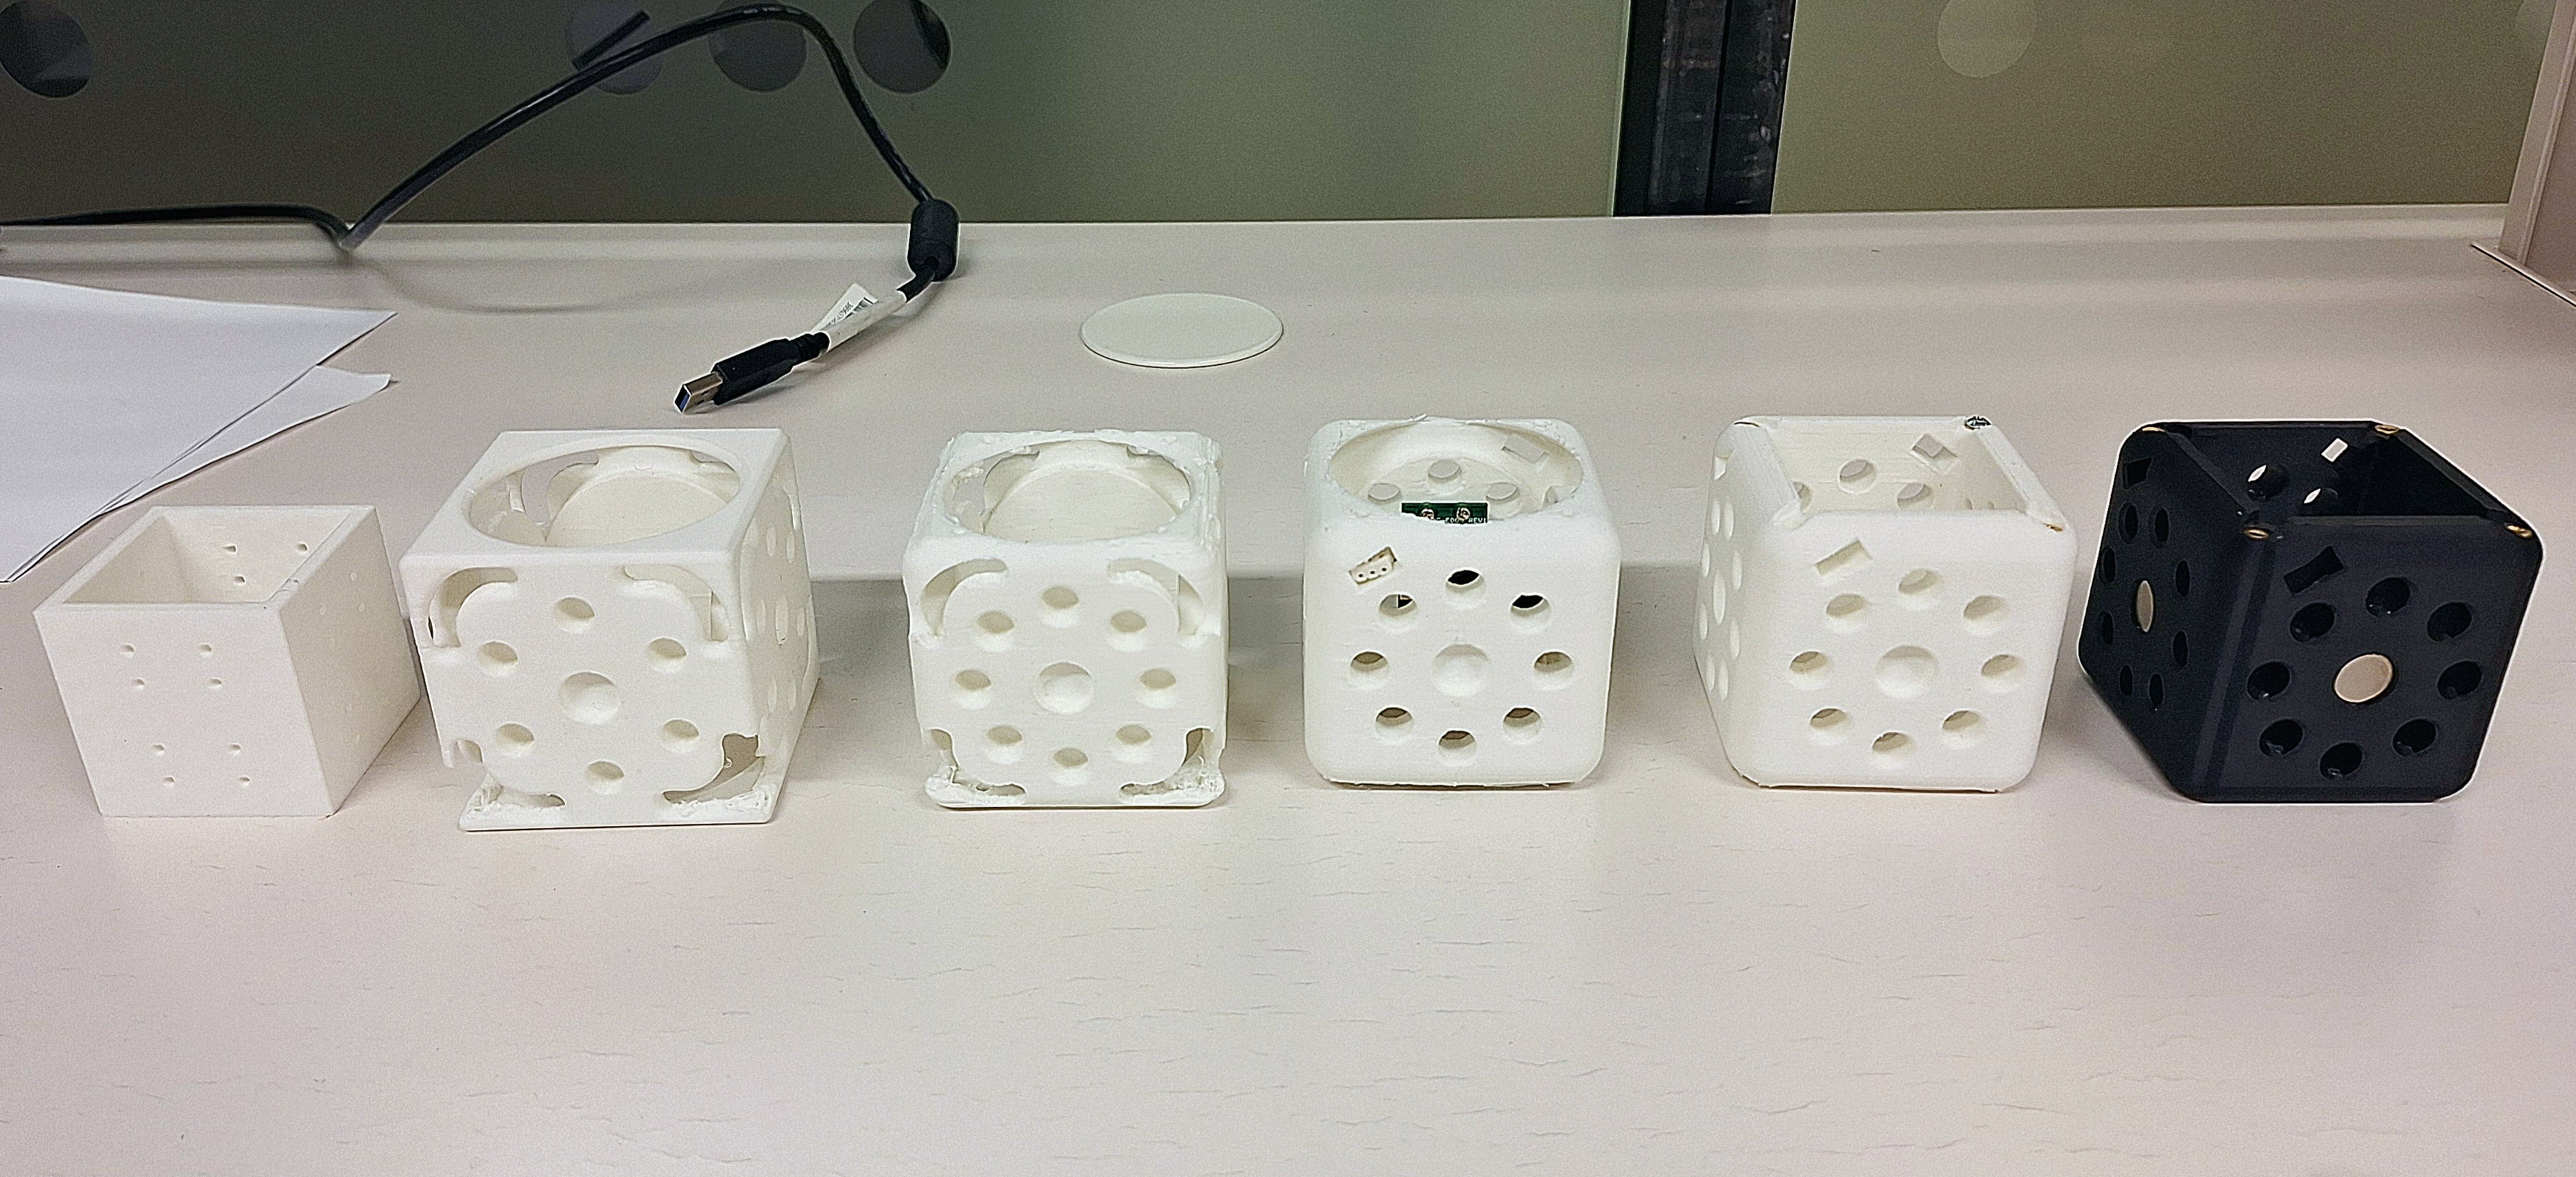
\includegraphics[width=1.01\linewidth]{images/image1.jpg}
       \\
       \small Evolution of gen. 1 to 7 of the Brick module

       \vspace{2em} % Space between rows

       % Row 2
       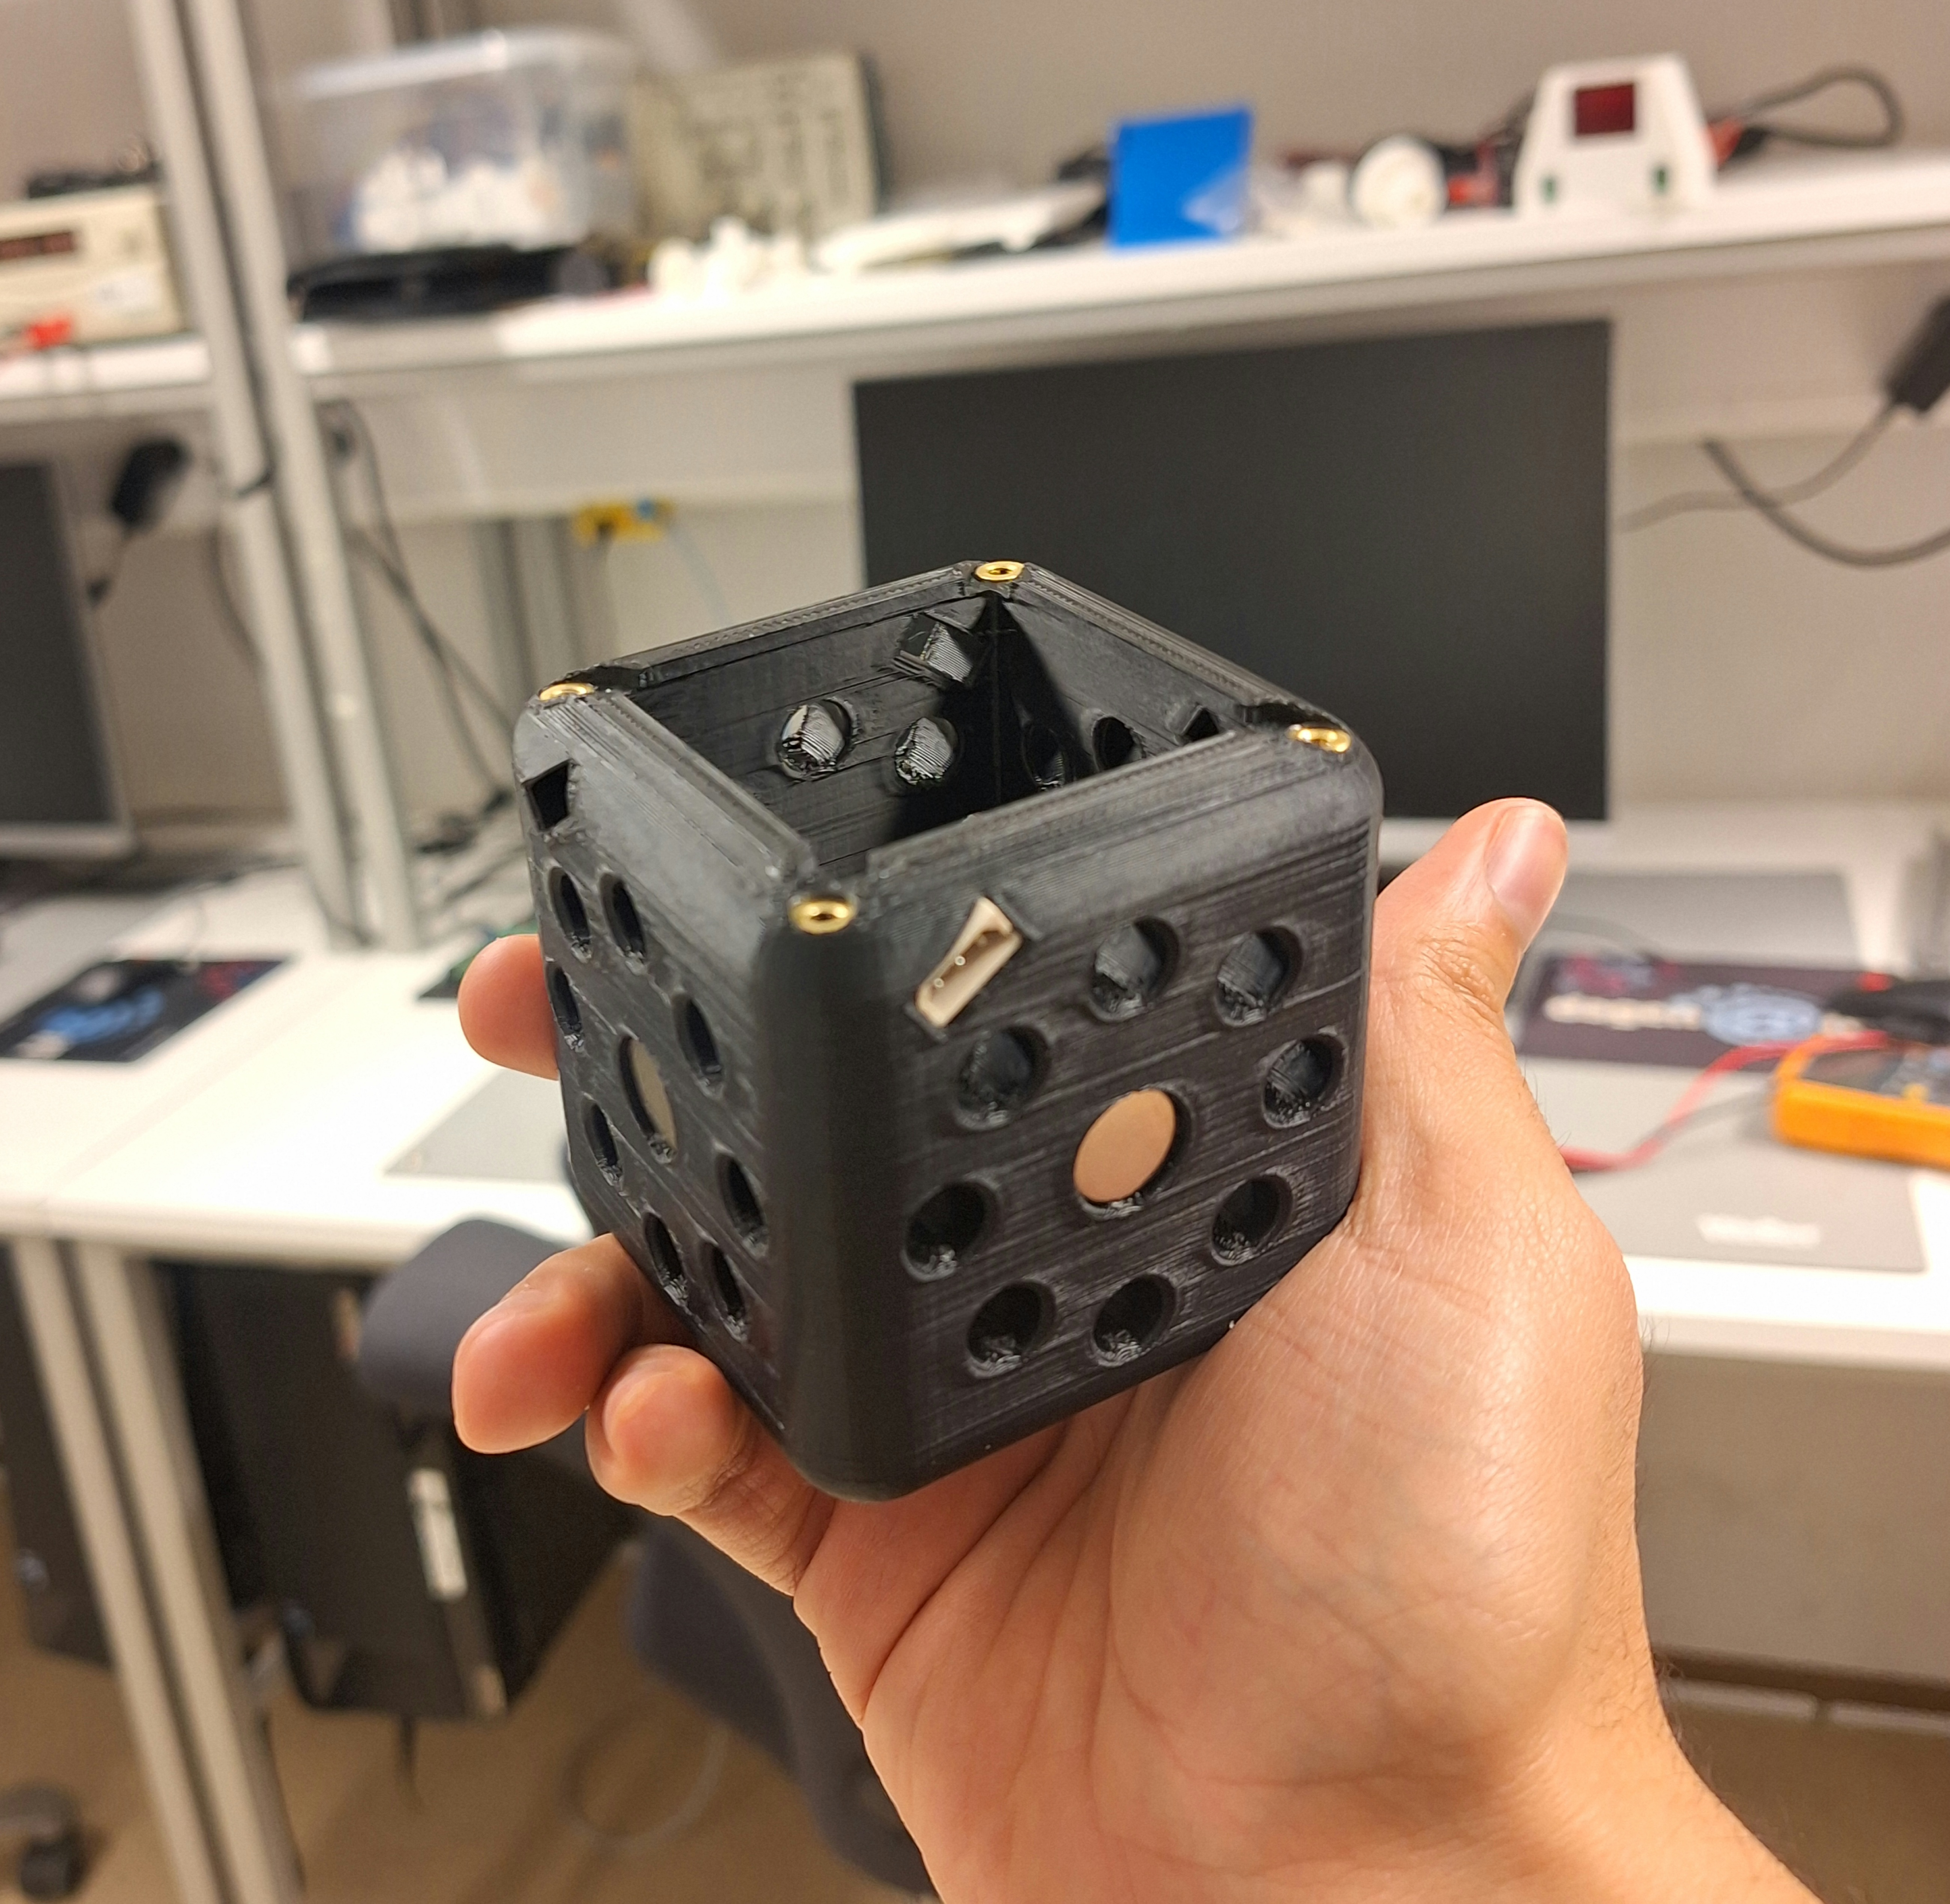
\includegraphics[width=0.47\linewidth]{images/image2a.jpg}
       \hspace{0.03\linewidth} % Space between images
       \includegraphics[width=0.47\linewidth]{images/image2b.jpg}
       \\
       \small The latest generation (gen. 7) of the Brick module

       \vspace{2em} % Space between rows

       % Row 3
       \includegraphics[width=0.47\linewidth]{images/image3a.jpg}
       \hspace{0.03\linewidth} % Space between images
       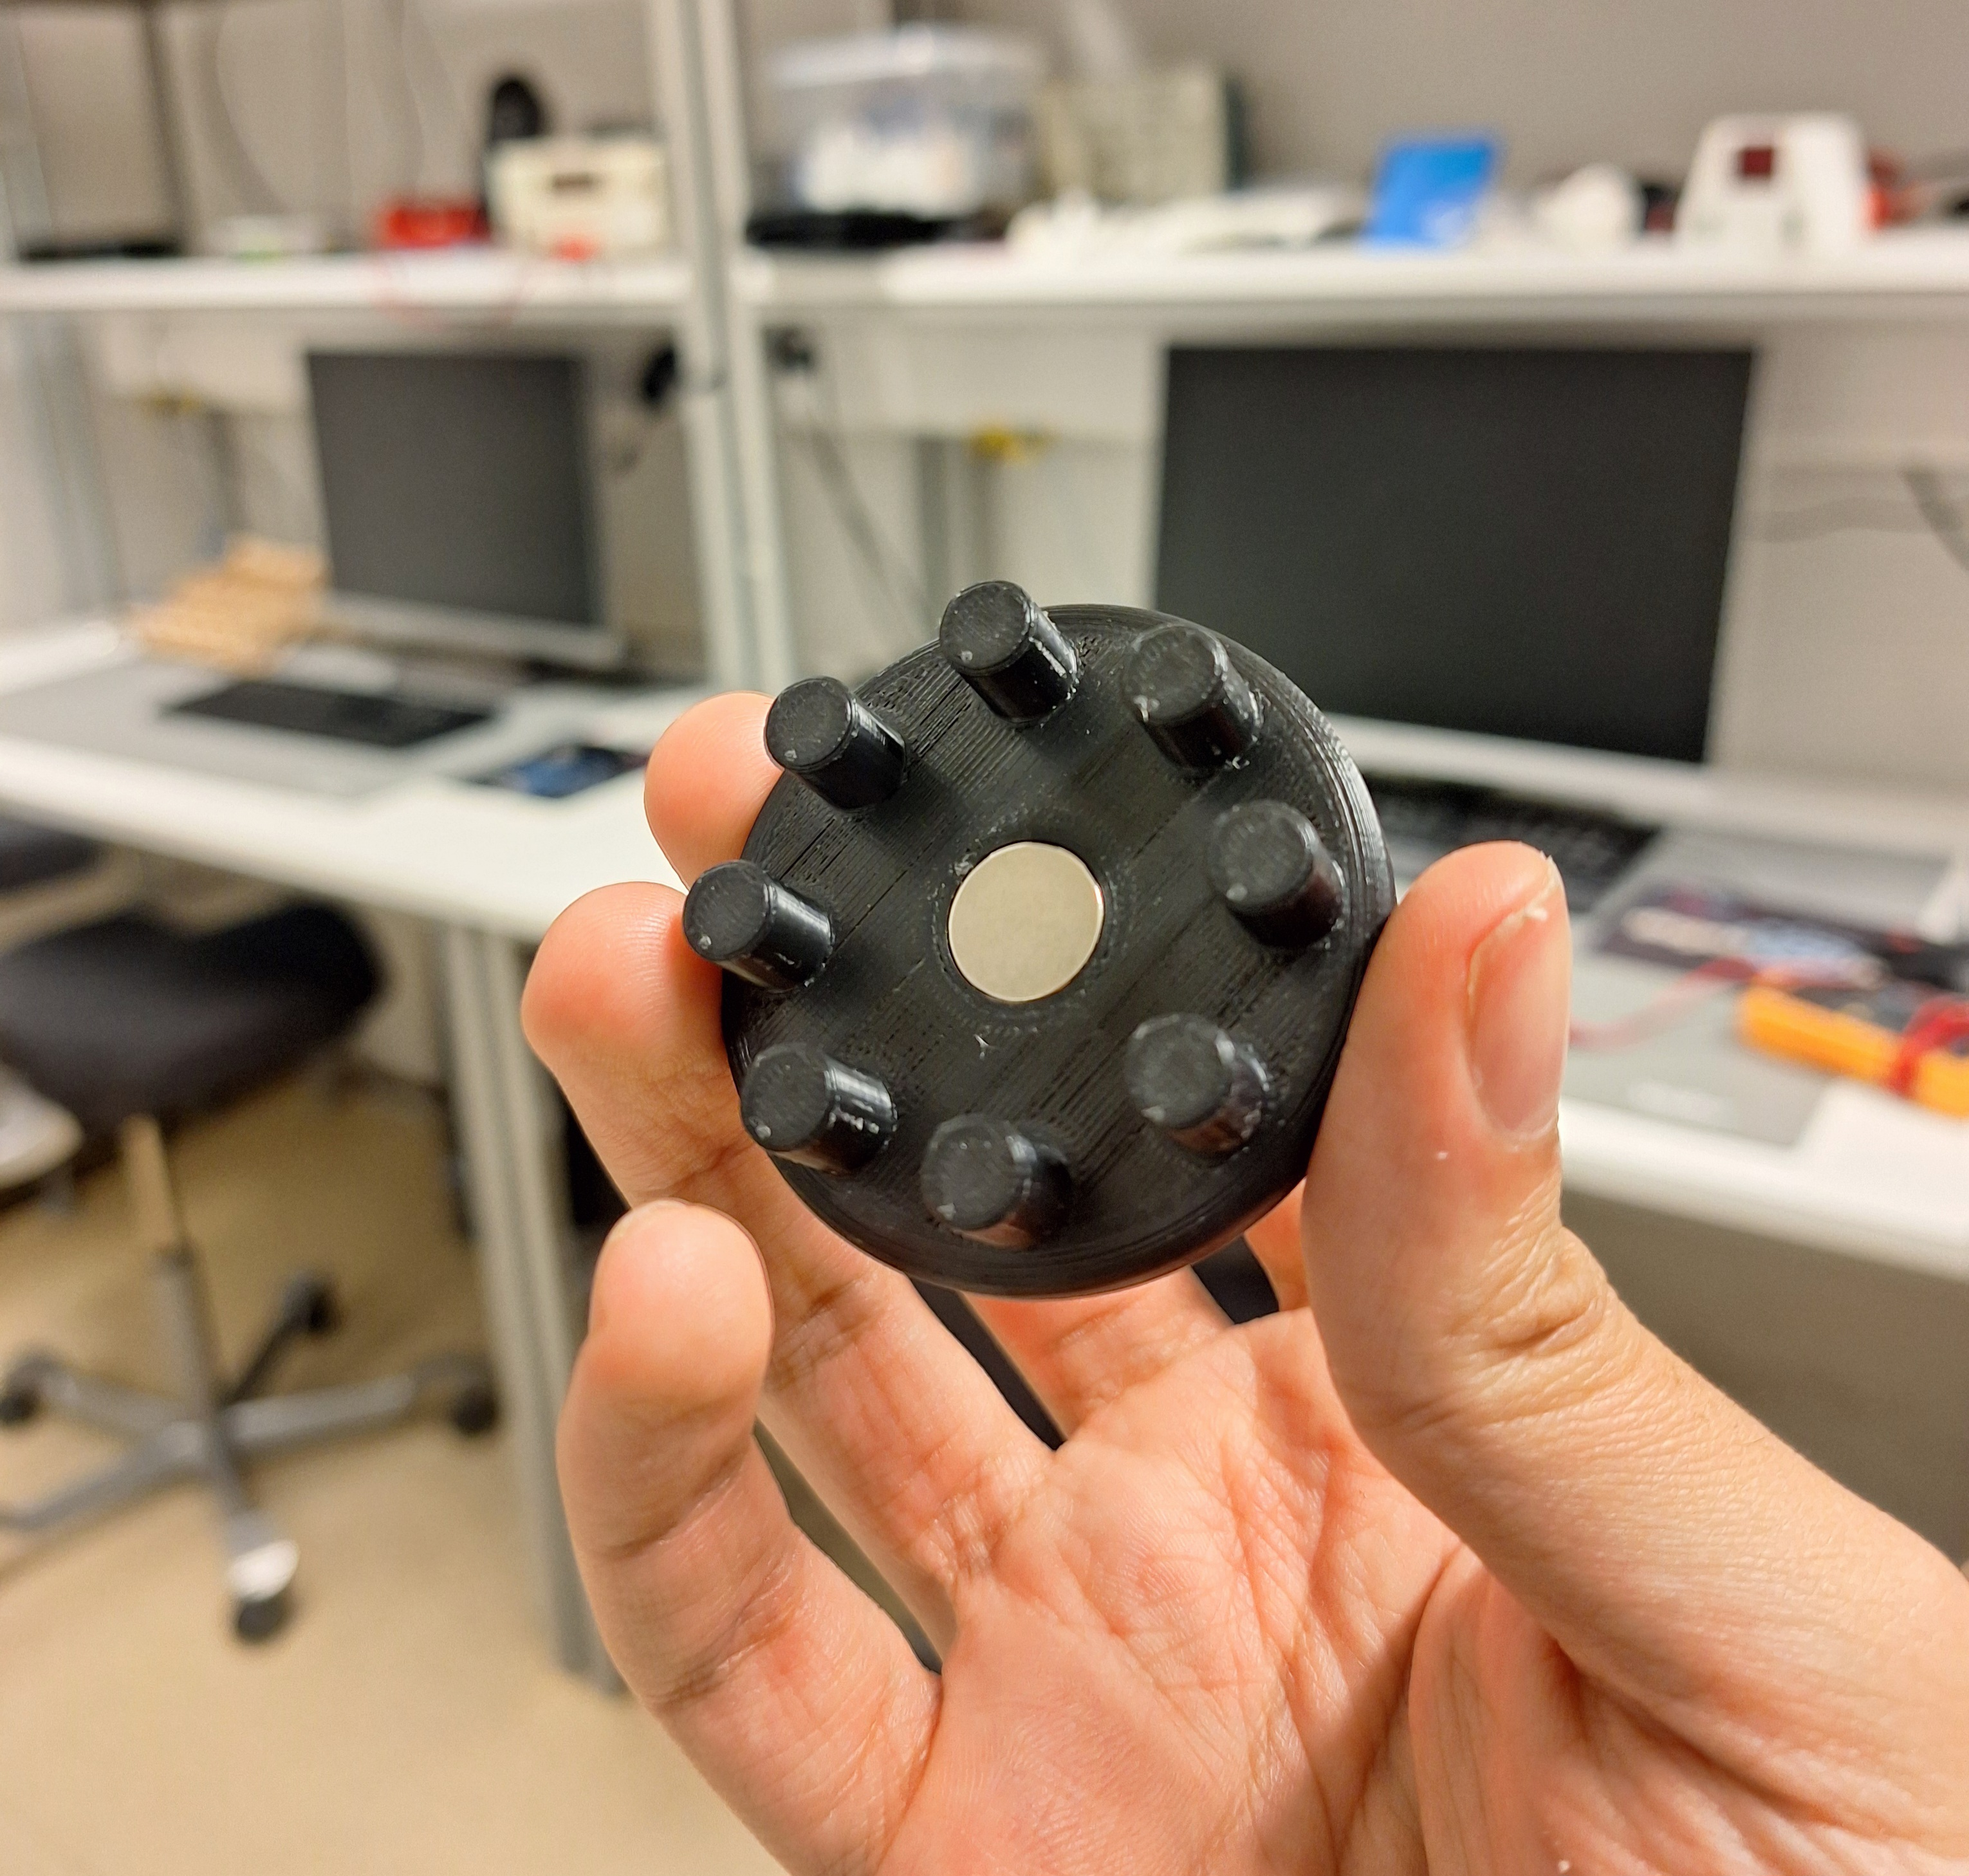
\includegraphics[width=0.47\linewidth]{images/image3b.jpg}
       \\
       \small The latest generation (gen. 7) of the Joint module

       \vspace{2em} % Space between rows

       % Row 4
       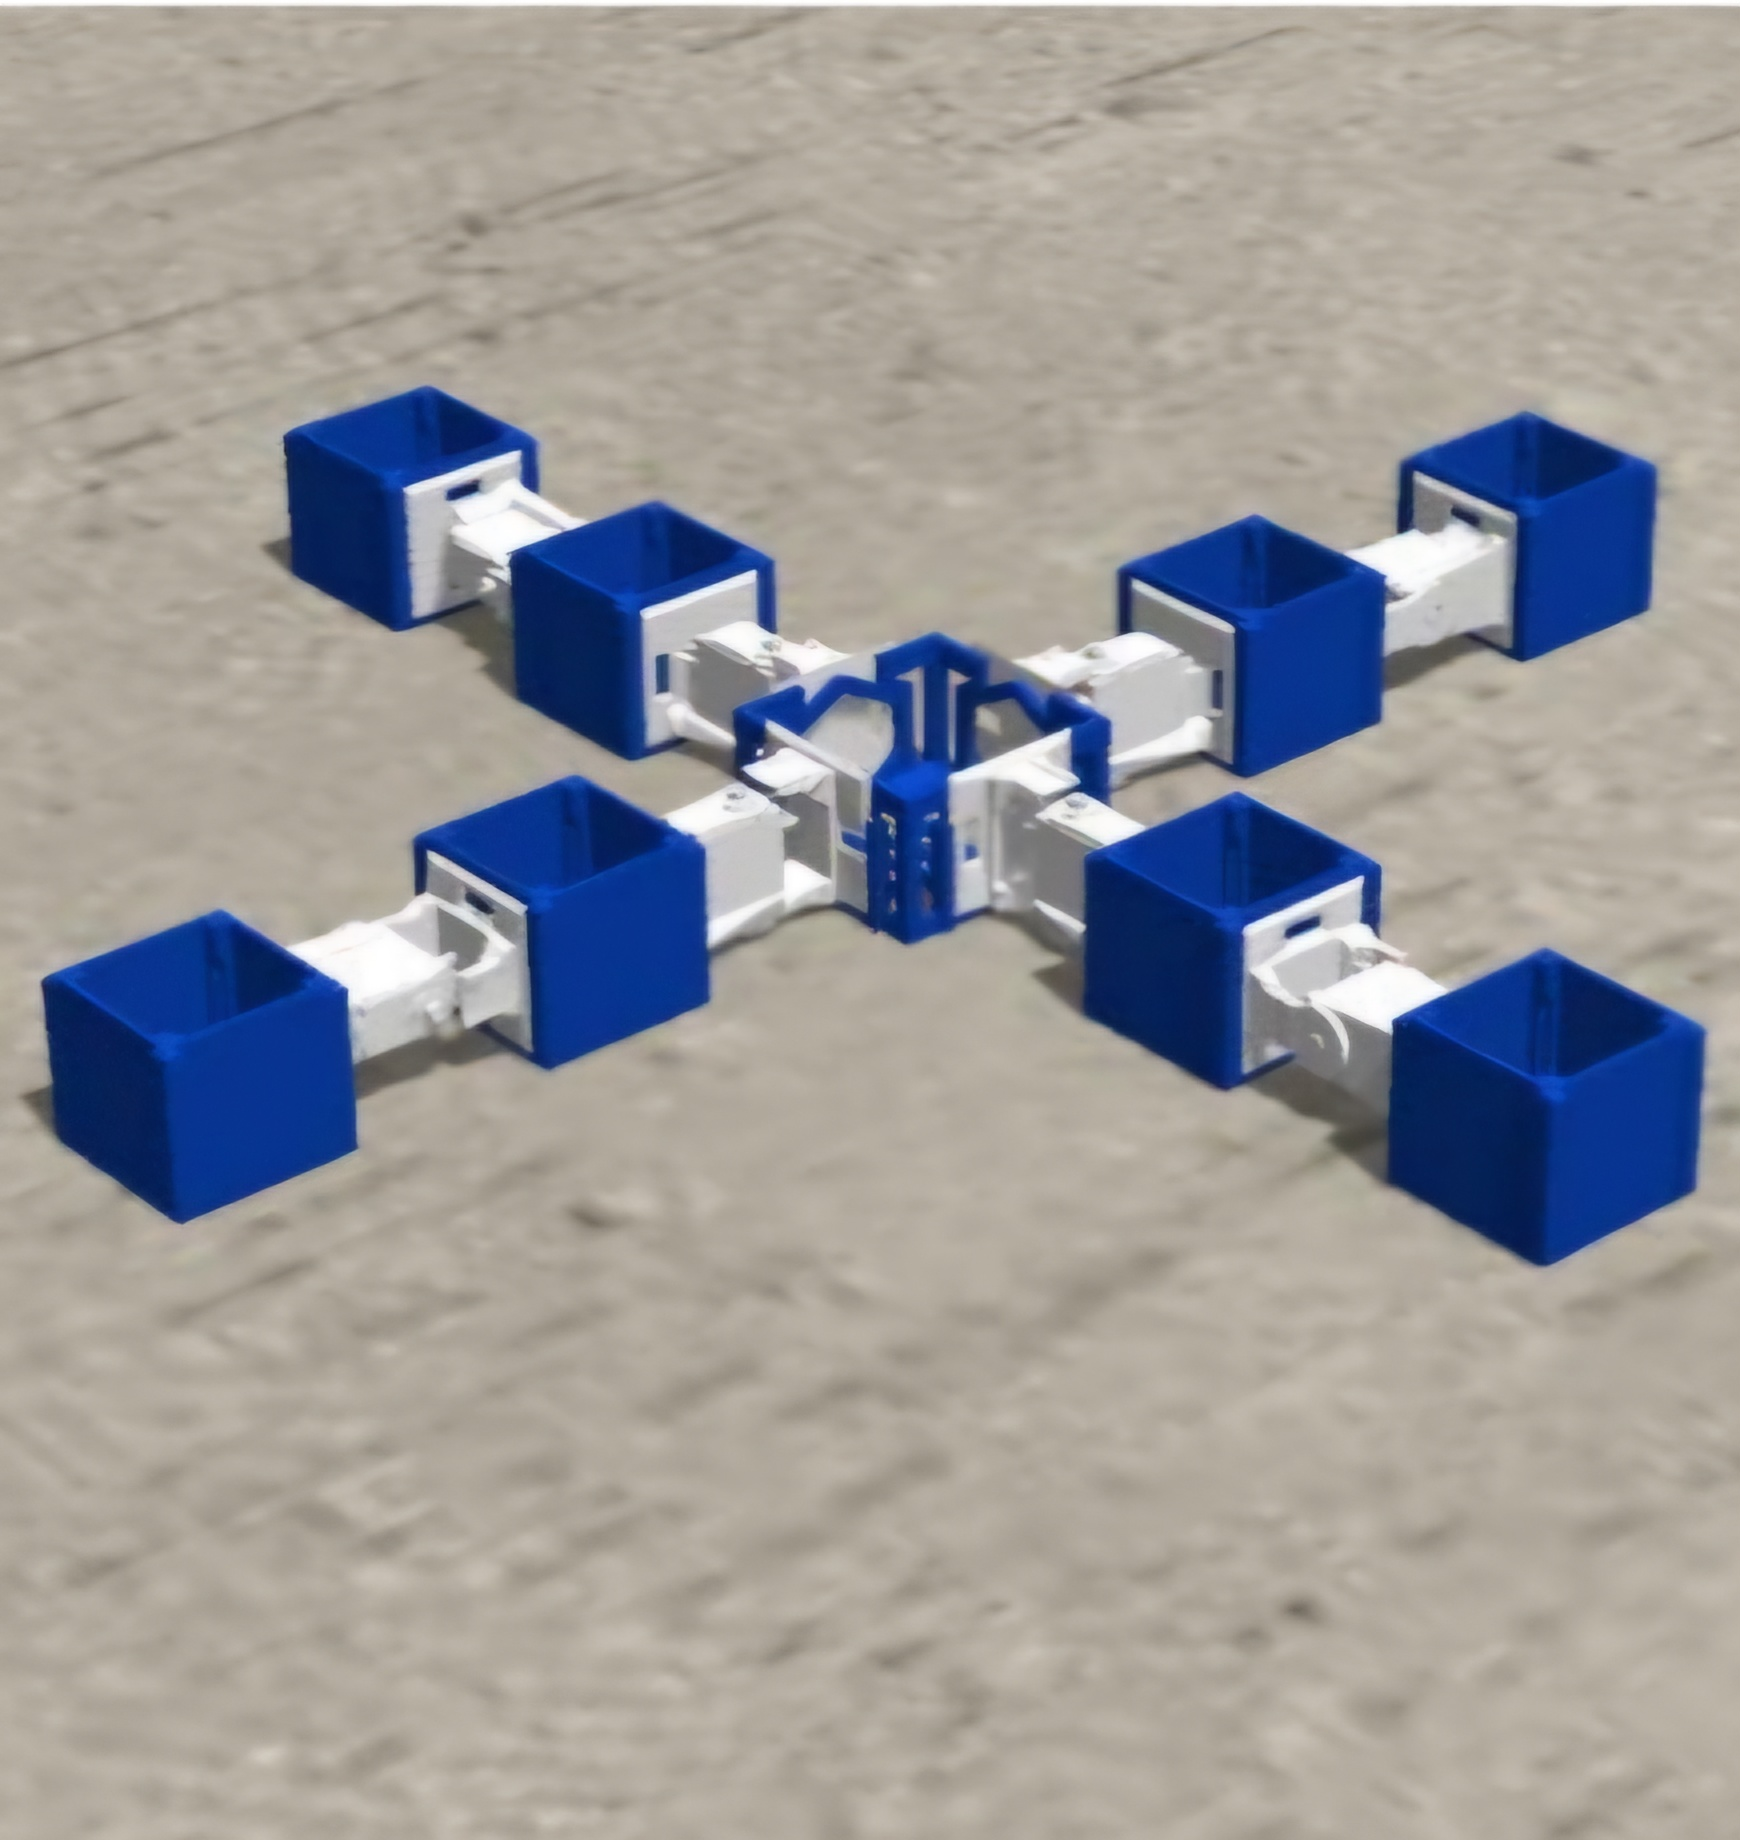
\includegraphics[width=0.47\linewidth]{images/image4a.jpg}
       \hspace{0.03\linewidth} % Space between images
       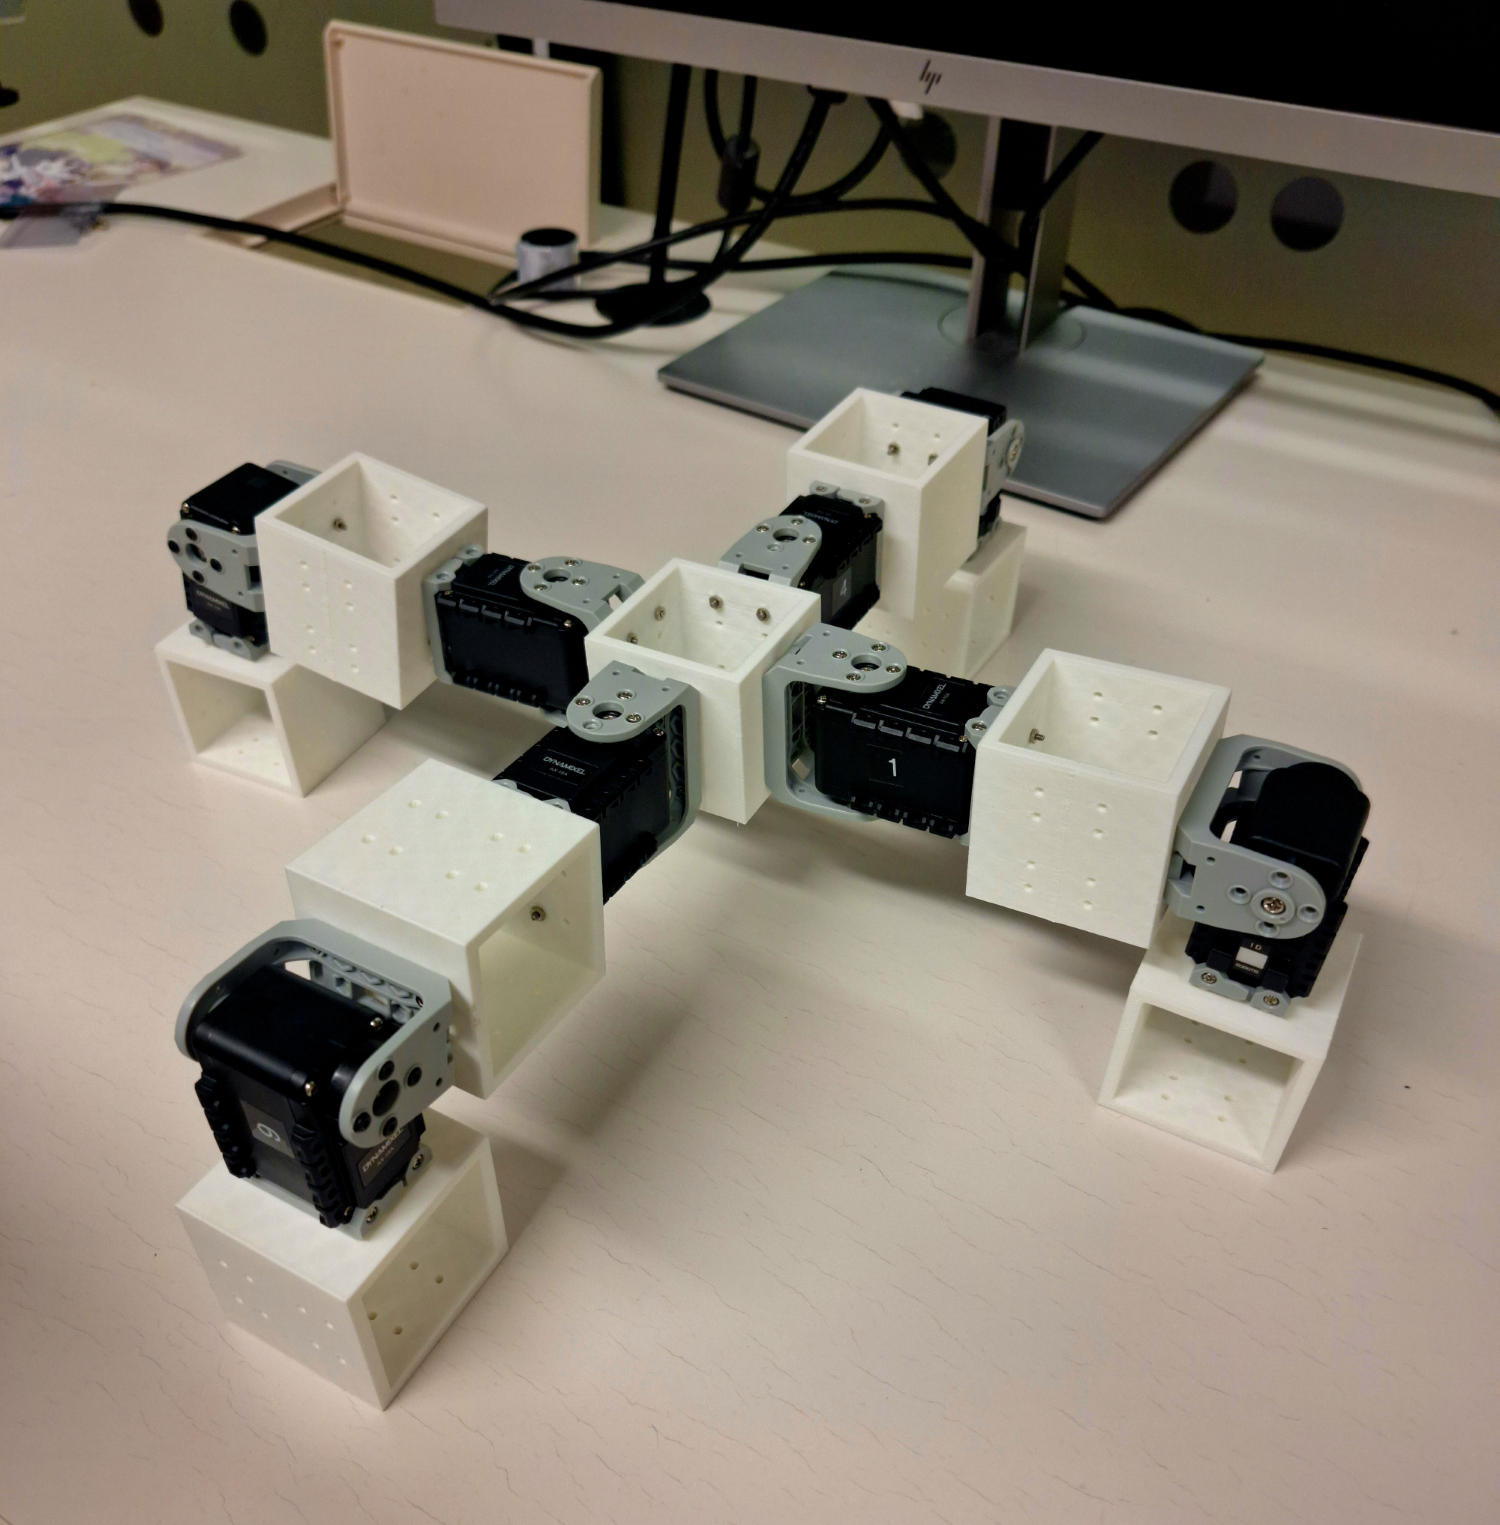
\includegraphics[width=0.47\linewidth]{images/2.png}
       \\
       \small Left: Revolve2 simulation of a spider robot
       \\ Right: Spider with 3D-printed gen. 1 modules

       \vspace{2em} % Space between rows

       % Row 5
       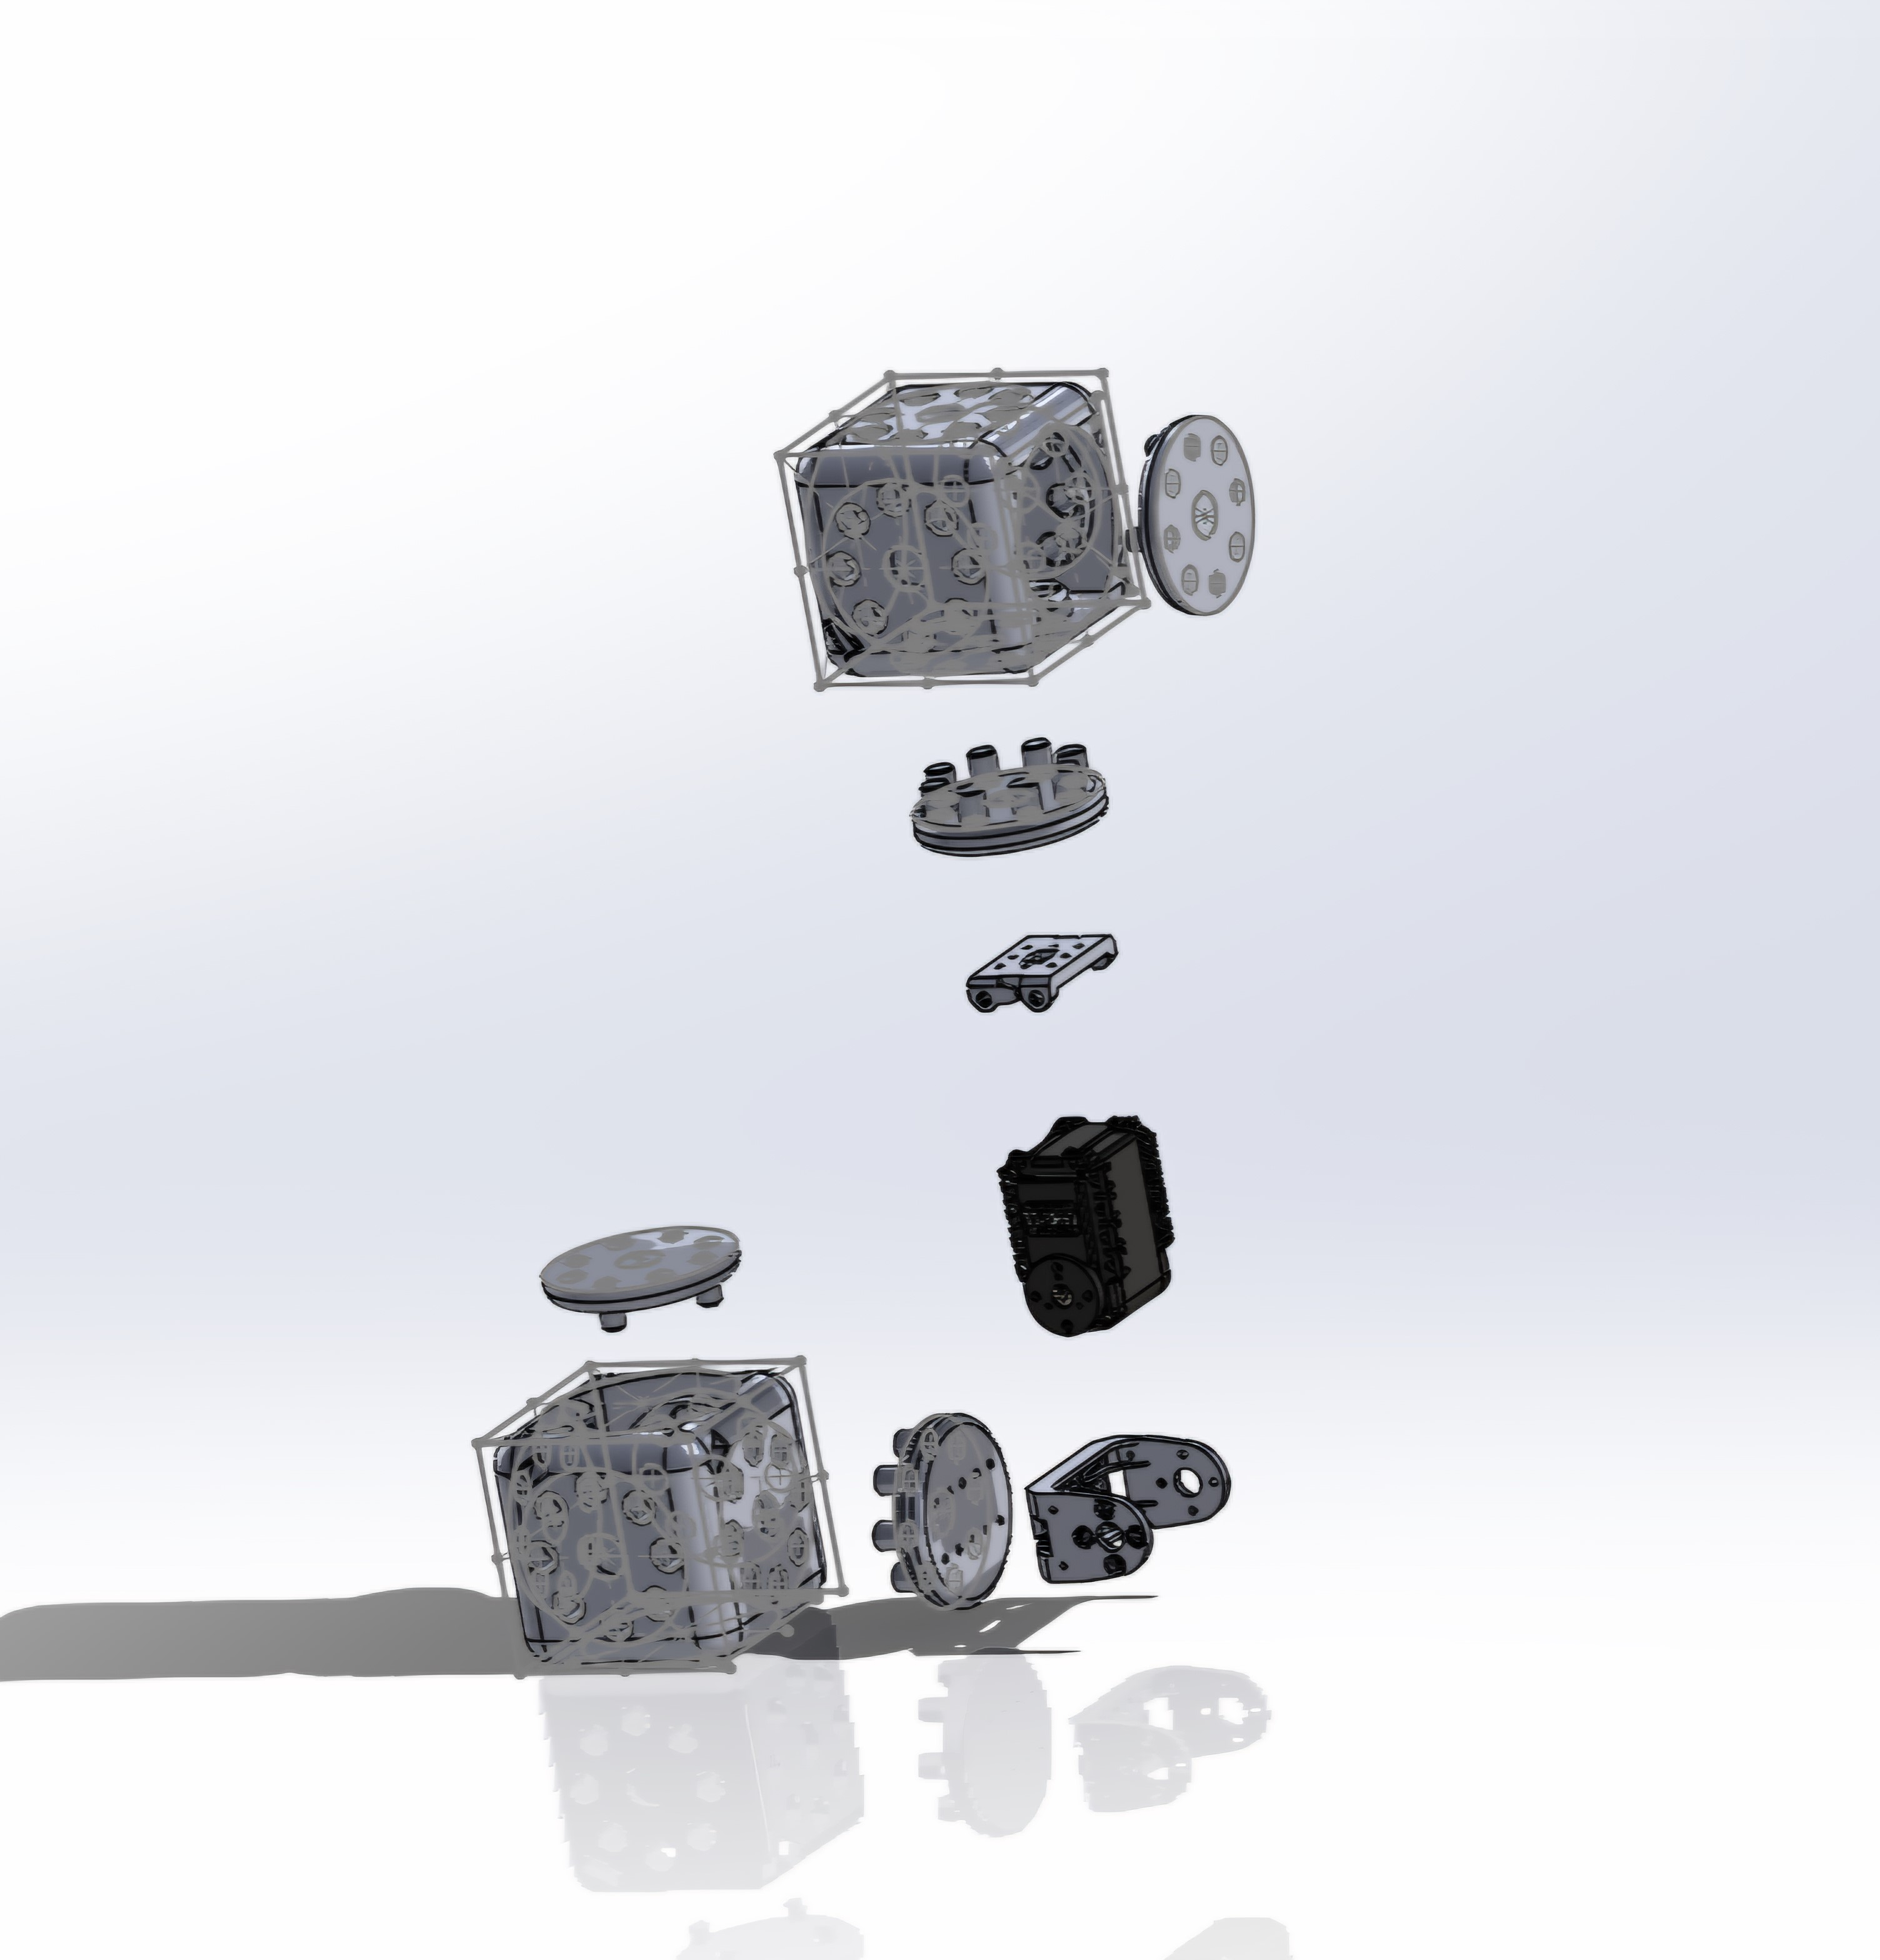
\includegraphics[width=0.47\linewidth]{images/image5a.jpg}
       \hspace{0.03\linewidth} % Space between images
       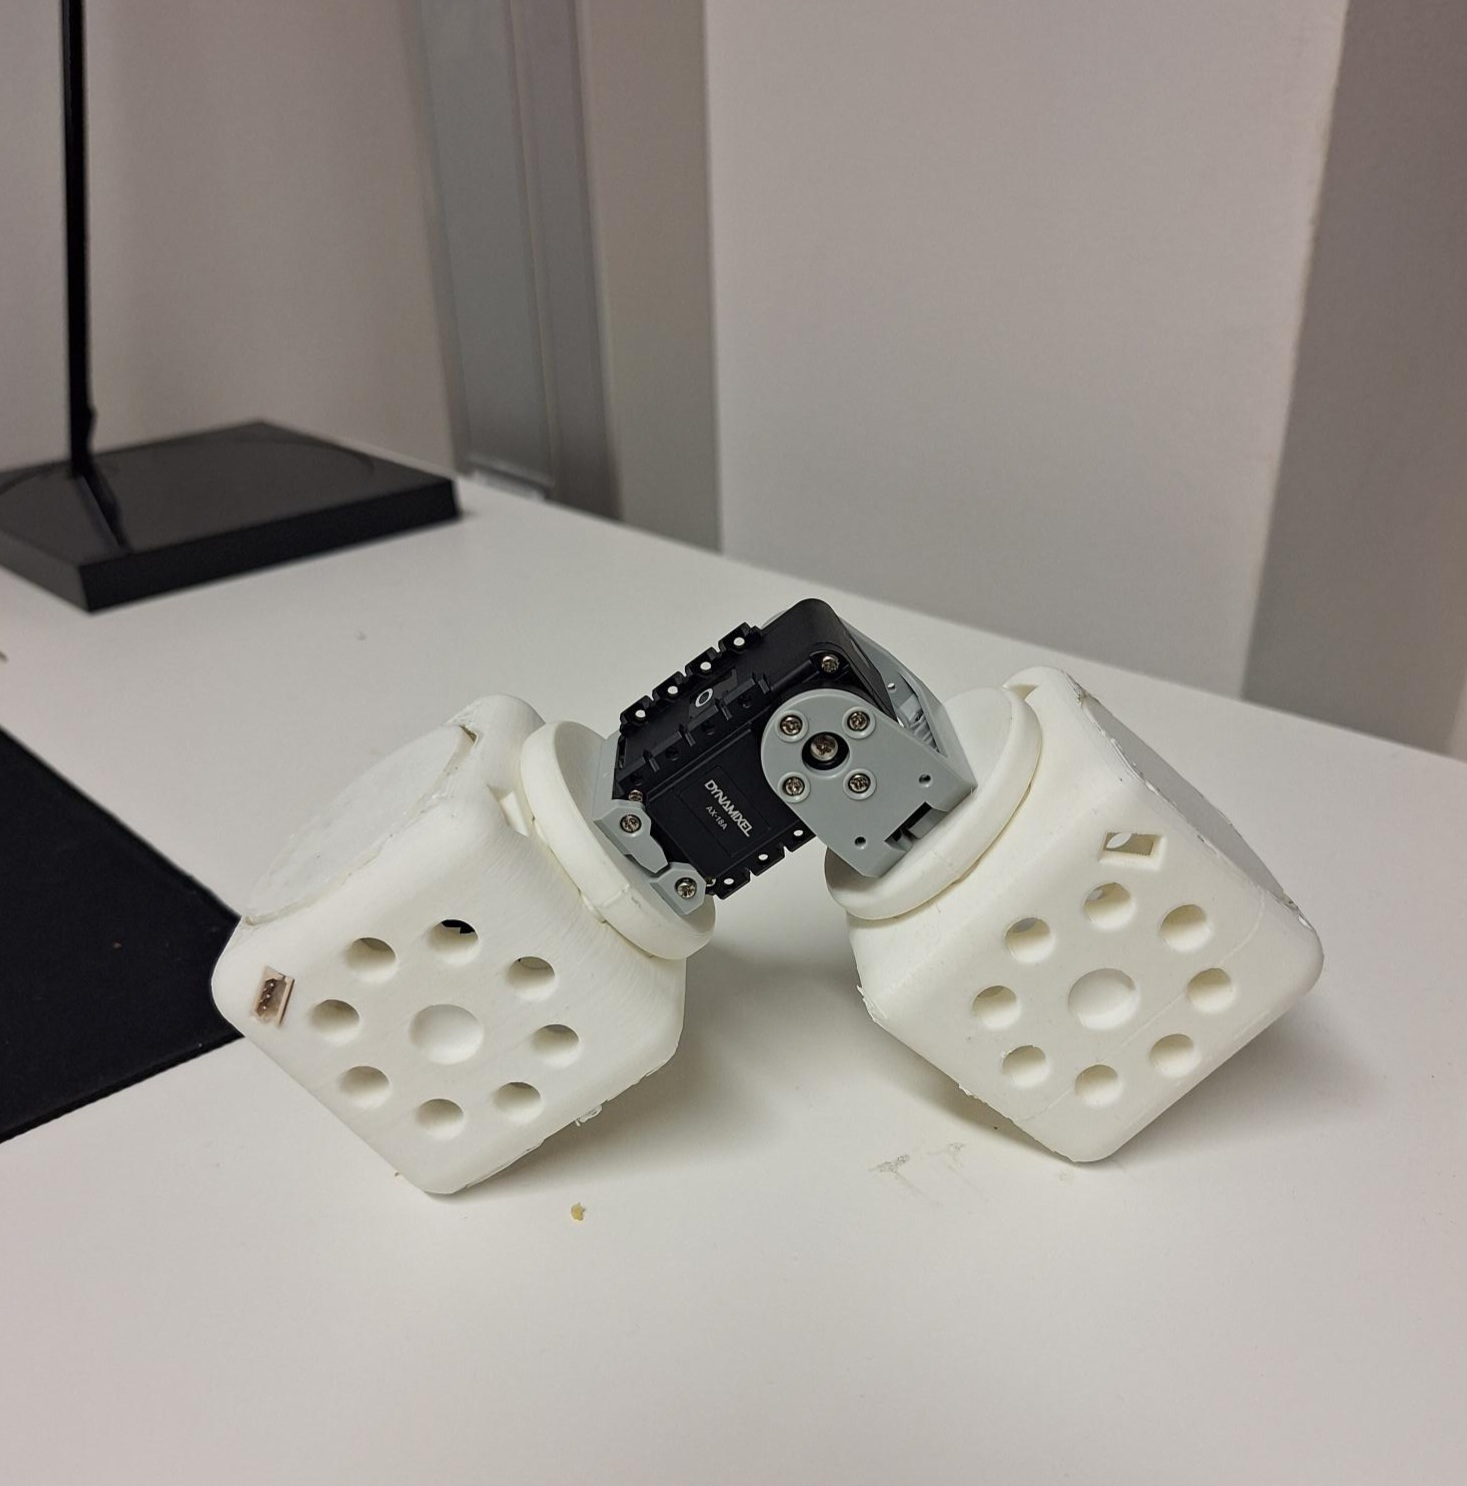
\includegraphics[width=0.47\linewidth]{images/image5b.jpg}
       \\
       \small Left: SolidWorks Exploded view of the modules \\Right: 3D-printed gen. 4 modules in a  worm config
   \end{center}

   If you are interested in collaboration on this project or have any questions feel free to contact me at amalmuda@ifi.uio.no

}

% footer
% generate qr code from https://www.qr-code-generator.com/ and replace qr_code.png
% default: barcode on the left
\makealtfooter{images/uni_logo.png}{images/qr-code.png}
% replace with this like for barcode on the right
%\makealtfooter{images/uni_logo.png}{images/qr-code.png}
\end{document}